\documentclass[12pt]{article}
\usepackage{tu-reports}

% ---- Fill out the following: ---- %
\authorfirst{FIRST-NAME} 
\authorlast{LAST-NAME}
\authorid{STUDENT-ID}
\theclass{COURSE ID-}{SECTION} 
\labname{LAB NAME}
\labgroup{GROUP NO.}
\labpartners{Group partners}
\labdate{LAB DATE}
\leftextra{}
\rightextra{}

\begin{document} 

\LabHeader

\section*{Introduction}
\lipsum[1-2]
\section*{Materials}
\lipsum[3-3]
\section*{Procedure}
\lipsum[4-5]
\subsection*{Part A}
\begin{figure}
	\centering
	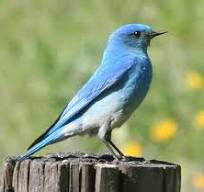
\includegraphics[width=0.7\linewidth]{bird.jpg}
	\caption{A bird.}
\end{figure}
\lipsum[10]
\subsection*{Part B}
\lipsum[11]

\section*{Results and Calculations}
\lipsum[6-6]
\subsection*{Part A}

\begin{align*}
	A &= \pi r^2 \\
	  &= \pi \frac{d}{2}^2
\end{align*}

\subsection*{Part B}

\begin{table}
	\centering
	\begin{tabular}{|c|c|c|c|}
		\hline
		A & B & C & D \\
		\hline
		1 & 2 & 3 & 4 \\
		\hline
		5 & 6 & 7 & 8 \\
		\hline
		9 & 10 & 11 & 12 \\
		\hline
	\end{tabular}
	\caption{Table for part B}
\end{table}

\section*{Conclusion}
\lipsum[7-8]
\pagebreak

\section*{Q/A}

\QA{This is a question?}{This is an answer.}
\QA{What is the meaning of life?}{The quick brown fox jumps over the lazy dog.}
\QA{How should I respond to criticism?}{\lipsum[1]}

\end{document}
